% Provenance (never printed): see sources/outline_sources.md (Year 3:
% fractionation and Rayleigh distillation in the water cycle;
% palaeothermometry; carbon and sulfur isotopes). Brief:
% sources/book5/BRIEFS.md, ch. 14. Curves from figdata/bachelor-3/
% rayleigh_distillation.py, lr04_d18o.py, carbon_mass_balance.py. Exercise
% and problem values in the Book 5 scratch calculator calc/ch14.py. Dome Ilse,
% its traverse and the marine core are invented.
\chapter{Geokimia Isotop Stabil}\label{ch:b3:stable-isotopes}

Salju yang turun di kubah-kubah tinggi lembaran es Antarktika Timur termasuk air
paling ringan di Bumi. Setiap molekulnya meninggalkan samudra sebagai uap, dan
dalam perjalanan ke pedalaman, udara kehilangan sebagian besar airnya sebagai salju, molekul berat
lebih dulu. Yang tersisa saat tiba bergantung pada seberapa banyak yang hilang, yang pada gilirannya bergantung pada
seberapa dingin udara itu menjadi. Karena itu, inti es adalah termometer, cangkang
kalsit termometer lain, dan karbon batu gamping ialah catatan tentang apa yang
dikubur biosfer. Bab ini menurunkan hukum di balik catatan-catatan itu dan
membacanya.

\begin{recall}
Nilai $\delta$, faktor fraksionasi $\alpha$, serta efek isotop kesetimbangan dan
efek isotop kinetik ada di volume universitas buku kimia. Standar
acuan VSMOW dan VPDB serta garis air meteorik ada di
volume Tahun 2, pada bab geokimia isotopnya; hukum fraksionasi
Rayleigh untuk unsur jejak ada di bab
diferensiasi magmatik; proksi iklim, efek volume es, dan termometer Mg/Ca
dibahas di bab arsip dan proksi iklim; sedangkan Maksimum Termal Paleosen--Eosen
ada di bab iklim sepanjang
waktu geologi; Peristiwa Oksidasi Besar ada di bab Bumi Prakambrium.
Fotosintesis dan reduksi sulfat oleh bakteri ada di buku biologi.
\end{recall}

\section{Fraksionasi antara dua fase}\label{sec:b3:stable-isotopes:fractionation}

Untuk dua fase A dan B dalam kesetimbangan isotop, $\alpha_{A-B} = R_A/R_B =
(1000 + \delta_A)/(1000 + \delta_B)$, dengan $R$ sebagai rasio isotop berat terhadap
isotop ringan. Uap air dan air cair memiliki $\alpha = 1.0098$ untuk oksigen-18
dan $1.084$ untuk deuterium pada \qty{20}{\celsius}, $1.0117$ dan $1.111$ pada
\qty{0}{\celsius}; es dan air pada \qty{0}{\celsius}, $1.0035$ dan $1.0208$.
Fase yang lebih berat selalu lebih terkondensasi, dan fraksionasi
membesar seiring turunnya suhu.
% ledger: kc98:alpha, kc98:standards

\begin{definition}[Selisih isotop]\label{def:b3:stable-isotopes:big-delta}
Yang disebut \emph{selisih isotop}\index{selisih isotop (delta kapital)}
antara dua fase adalah $\Delta_{A-B} = \delta_A - \delta_B$, dalam per mil.
\end{definition}

\begin{proposition}[Selisih isotop dan faktor fraksionasi]
\label{prop:b3:stable-isotopes:big-delta}
Untuk $\alpha$ mendekati 1 dan nilai $\delta$ yang kecil,
\[
\Delta_{A-B} \approx 1000\ln\alpha_{A-B} \approx 1000(\alpha_{A-B} - 1).
\]
\end{proposition}

\begin{proof}
$1000\ln\alpha = 1000\ln(1 + \delta_A/1000) - 1000\ln(1 + \delta_B/1000)$, dan
$1000\ln(1 + x/1000) = x - x^2/2000 + \dots$, sehingga $1000\ln\alpha = \delta_A -
\delta_B - (\delta_A^2 - \delta_B^2)/2000 + \dots$. Akhirnya $\ln\alpha \approx
\alpha - 1$ untuk $\alpha$ dekat 1.
\end{proof}

Galatnya adalah $(\delta_A^2 - \delta_B^2)/2000$: sebagian kecil per mil pada
nilai samudra, hampir satu per mil antara samudra dan salju ringan
es kutub.
Besaran $1000\ln\alpha$ itulah yang dikaitkan teori dengan suhu: ia
berubah hampir sebanding dengan $1/T^2$ pada suhu tinggi dan dengan $1/T$ pada suhu rendah,
dan kalibrasi biasanya ditulis dalam bentuk itu. Untuk es dan uap, misalnya,
\[
\ln\alpha^{18}_{\mathrm{ice-v}} = \frac{11.839}{T} - 0.028224, \qquad
\ln\alpha^{\mathrm D}_{\mathrm{ice-v}} = \frac{16288}{T^2} - 0.0934,
\]
dengan $T$ dalam kelvin.
% ledger: gkinis14:alpha-ice, kc98:standards

\begin{definition}[Fraksionasi bergantung massa dan tak bergantung massa]\label{def:b3:stable-isotopes:mif}
Unsur dengan tiga isotop atau lebih memiliki \emph{fraksionasi
bergantung massa}\index{fraksionasi bergantung massa} jika fraksionasi
rasio isotopnya sebanding dengan selisih massanya, sebagaimana ditentukan oleh
massanya; jika tidak, unsur itu memiliki \emph{fraksionasi
tak bergantung massa}\index{fraksionasi tak bergantung massa}, diukur dari simpangan
dari garis bergantung massa, misalnya $\Delta^{33}\mathrm S = \delta^{33}\mathrm S
- 0.515\,\delta^{34}\mathrm S$.
\end{definition}

Untuk oksigen, fraksionasi $^{17}\mathrm O/^{16}\mathrm O$ kira-kira 0.52 kali
dari $^{18}\mathrm O/^{16}\mathrm O$, mendekati perbandingan selisih massanya, 1 banding 2;
untuk belerang, $\delta^{33}\mathrm S = 0.515\,\delta^{34}\mathrm S$. \omterm{def:b3:stable-isotopes:mif}{Fraksionasi
tak bergantung massa} jarang terjadi: ditemukan pada meteorit, ozon stratosfer, dan
belerang Arkean.
% ledger: white13c9:mdf, white13c9:s-mif

\section{Distilasi Rayleigh dalam siklus air}\label{sec:b3:stable-isotopes:rayleigh}

Massa udara yang mendingin membentuk tetesan awan atau kristal salju, yang jatuh dan
meninggalkan udara. Setiap kondensat lebih kaya isotop berat daripada uap, sehingga
uap yang tersisa makin ringan, dan kondensat berikutnya, dalam kesetimbangan dengannya, juga
lebih ringan.

\begin{proposition}[Distilasi Rayleigh]\label{prop:b3:stable-isotopes:rayleigh-distillation}
Misalkan suatu reservoar uap kehilangan airnya melalui kondensat, masing-masing langsung dikeluarkan begitu
terbentuk dalam kesetimbangan dengan uap. Jika $f$ adalah fraksi uap yang
tersisa dan $\alpha$ faktor fraksionasi kondensat--uap, maka
rasio uap mengikuti $\mathrm d\ln R_v = (\alpha - 1)\,\mathrm d\ln f$. Untuk
$\alpha$ konstan, ini disebut \emph{distilasi
Rayleigh}\index{distilasi Rayleigh}:
\[
\frac{R_v}{R_{v,0}} = f^{\,\alpha - 1}, \qquad
\delta_v = (1000 + \delta_{v,0})\,f^{\,\alpha - 1} - 1000,
\]
dan kondensat yang terbentuk pada $f$ memiliki $\delta_c = \alpha(1000 + \delta_v) - 1000$.
\end{proposition}

\begin{proof}
Misalkan $N$ adalah jumlah molekul uap (hampir semuanya ringan) dan $N R_v$
jumlah molekul yang berat. Jika $\mathrm dN < 0$ molekul kondensat dihilangkan,
maka $\alpha R_v\,\mathrm dN$ molekul berat ikut hilang: $\mathrm d(NR_v) = \alpha
R_v\,\mathrm dN$. Dengan demikian $N\,\mathrm dR_v = (\alpha - 1)R_v\,\mathrm dN$, yakni
hukum diferensial dengan $f = N/N_0$. Untuk $\alpha$ konstan, hukum ini terintegrasi
menjadi hukum pangkat.
\end{proof}

Jika $\alpha$ bergantung pada suhu, $\ln(R_v/R_{v,0}) = \int(\alpha - 1)\,
\mathrm d\ln f$ sepanjang lintasan. Untuk massa udara yang didinginkan pada tekanan tetap,
uap yang dapat ditampungnya ditentukan oleh tekanan jenuh, sehingga $f =
e_s(T)/e_s(T_0)$, yang diberikan oleh kurva sublimasi es di bawah
\qty{0}{\celsius}. Gambar berikut mengintegralkan hukum ini untuk massa udara yang
uapnya mulai pada \qty{0}{\celsius} dengan asumsi $\delta^{18}\mathrm O = -20$
dan $\delta\mathrm D = \qty{-150}{\permil}$. Uap nyata di atas samudra lebih
ringan daripada yang dihasilkan kesetimbangan dengan air laut, yaitu sekitar $-13$ alih-alih
\qty{-9}{\permil} untuk oksigen-18, karena penguapan sebagian bersifat kinetik.
% ledger: iapws:melt-subl, gkinis14:alpha-ice, white13c9:rayleigh

\begin{definition}[Kelebihan deuterium]\label{def:b3:stable-isotopes:d-excess}
Yang disebut \emph{kelebihan deuterium}\index{kelebihan deuterium} dari sampel air adalah $d =
\delta\mathrm D - 8\,\delta^{18}\mathrm O$, dalam per mil.
\end{definition}

Presipitasi dari benua-benua di belahan bumi utara berada pada garis
$\delta\mathrm D = 8.0\,\delta^{18}\mathrm O + 10$: \omterm{def:b3:stable-isotopes:d-excess}{kelebihan deuteriumnya} sekitar
\qty{10}{\permil}. Kemiringan 8 mendekati rasio fraksionasi kesetimbangan
kedua isotop dalam kondensasi. Kelebihan 10, bukan 0,
mencatat penguapan kinetik dari samudra, dan kelebihan suatu sampel
mengukur seberapa jauh dari kesetimbangan air itu menguap.
% ledger: dansgaard64:effects, kc98:mwl

\begin{omfigure}
\begin{tikzpicture}
\begin{groupplot}[group style={group size=2 by 1, horizontal sep=1.6cm},
  omrecord, width=0.47\linewidth, height=0.42\linewidth, title style={font=\small},
  tick label style={font=\scriptsize}, label style={font=\small},
  legend style={font=\scriptsize, legend cell align=left}]
\nextgroupplot[title={(a) sepanjang lintasan pendinginan},
  xlabel={suhu kondensasi (\unit{\celsius})}, ylabel={$\delta^{18}\mathrm O$ (\unit{\permil})},
  xmin=-55, xmax=0, ymin=-130, ymax=0, x dir=reverse,
  legend style={at={(0.03,0.03)}, anchor=south west}]
% computed in figdata/bachelor-3/rayleigh_distillation.py
\addplot[omDef, thick, densely dashed] table[x=t, y=d18v] {figdata/out/bachelor-3-rayleigh_distillation-curve.dat};
\addlegendentry{uap}
\addplot[omDef, thick] table[x=t, y=d18s] {figdata/out/bachelor-3-rayleigh_distillation-curve.dat};
\addlegendentry{salju}
\addplot[red!70!black, only marks, mark=*, mark size=1.6pt] table[x=t, y=d18s] {figdata/out/bachelor-3-rayleigh_distillation-stations.dat};
\addlegendentry{stasiun}
\nextgroupplot[title={(b) salju pada plot $\delta\mathrm D$--$\delta^{18}\mathrm O$},
  xlabel={$\delta^{18}\mathrm O$ (\unit{\permil})}, ylabel={$\delta\mathrm D$ (\unit{\permil})},
  xmin=-110, xmax=0, ymin=-700, ymax=0,
  legend style={at={(0.97,0.03)}, anchor=south east}]
\addplot[omDef, thick] table[x=d18s, y=dDs] {figdata/out/bachelor-3-rayleigh_distillation-curve.dat};
\addlegendentry{model salju}
\addplot[black, densely dotted, domain=-110:0, samples=2] {8*x + 10};
\addlegendentry{$\delta\mathrm D = 8\,\delta^{18}\mathrm O + 10$}
\addplot[red!70!black, only marks, mark=*, mark size=1.6pt, forget plot] table[x=d18s, y=dDs] {figdata/out/bachelor-3-rayleigh_distillation-stations.dat};
\end{groupplot}
\end{tikzpicture}

\par\smallskip{\small \omterm{prop:b3:stable-isotopes:rayleigh-distillation}{Distilasi Rayleigh} untuk massa udara yang didinginkan pada
tekanan tetap dari \qty{0}{\celsius}, dengan faktor fraksionasi es--uap
dan fraksi uap yang tersisa dibaca dari kurva sublimasi es. (a) Uap
(garis putus-putus) dan salju (garis penuh) makin ringan kian cepat; titik-titik itu
adalah tiga stasiun pada soal akhir pekan. (b) Salju model tetap dekat dengan
garis air meteorik hingga sekitar \qty{-30}{\permil} untuk oksigen-18, lalu naik
di atasnya.}\label{fig:b3:stable-isotopes:rayleigh}
\end{omfigure}
% ledger: kc98:mwl


\begin{definition}[Efek suhu, efek jumlah, dan efek benua]\label{def:b3:stable-isotopes:effects}
Yang disebut \emph{efek suhu}\index{efek suhu (isotopik)} adalah
penurunan $\delta^{18}\mathrm O$ dan $\delta\mathrm D$ presipitasi terhadap
suhu lokal. Yang disebut \emph{efek jumlah}\index{efek jumlah} adalah
penurunan keduanya terhadap jumlah hujan, di daerah tropis. Yang disebut \emph{efek
benua}\index{efek benua} adalah penurunan keduanya ke arah pedalaman, pada
suhu tertentu.
\end{definition}

Ketiganya adalah \omterm{prop:b3:stable-isotopes:rayleigh-distillation}{distilasi Rayleigh} yang diamati dari permukaan. Pada lintang tinggi
\omterm{def:b3:stable-isotopes:effects}{efek suhu} mendominasi: rata-rata tahunan stasiun Greenland dan Atlantik
Utara mengikuti $\delta^{18}\mathrm O = 0.69\,t - 13.6$ dan $\delta\mathrm D =
5.6\,t - 100$ (dalam per mil, dengan $t$ suhu permukaan rata-rata tahunan dalam
\unit{\celsius}). Di daerah tropis \omterm{def:b3:stable-isotopes:effects}{efek jumlah} mendominasi: pada satu
pulau samudra, curah hujan bulanan kehilangan sekitar \qty{1.6}{\permil} oksigen-18 untuk setiap
\qty{100}{mm} hujan tambahan. Model sederhana pada gambar di atas memberikan kemiringan yang lebih curam,
sekitar \qty{1.6}{\permil} per derajat suhu kondensasi. Kedua kemiringan
itu tidak dapat dibandingkan langsung: permukaan lembaran es lebih dingin
daripada udara tempat salju terbentuk, dan model mengabaikan pencampuran massa
udara serta efek kinetik pembentukan salju, sehingga kemiringan terhadap suhu
permukaan hanya dikalibrasi, bukan dihitung.
% ledger: dansgaard64:effects

\section{Paleotermometri}\label{sec:b3:stable-isotopes:palaeothermometry}

\begin{definition}[Paleotermometri, persamaan paleosuhu]
\label{def:b3:stable-isotopes:palaeothermometry}
Yang disebut \emph{paleotermometri}\index{paleotermometri} adalah pengukuran suhu masa lalu
dari komposisi bahan yang terbentuk saat itu. Sebuah
\emph{persamaan paleosuhu}\index{persamaan paleosuhu} adalah
hubungan terkalibrasi antara suhu pembentukan suatu mineral dan
fraksionasinya dengan air tempat ia tumbuh.
\end{definition}

Untuk kalsit yang mengendap perlahan dari air, satu kalibrasi memberikan
\[
1000\ln\alpha_{\mathrm{calcite-water}} = 18.03\,\frac{10^3}{T} - 32.42,
\]
dengan kedua nilai $\delta$ pada skala VSMOW. Karbonat dilaporkan pada skala
VPDB, dikonversi dengan $\delta^{18}\mathrm O_{\mathrm{VPDB}} =
0.97001\,\delta^{18}\mathrm O_{\mathrm{VSMOW}} - 29.99$. Dekat \qty{5}{\celsius}, fraksionasi
turun sekitar \qty{0.23}{\permil} per derajat pemanasan.
% ledger: isogeochem:ko97

\begin{method}[Paleosuhu karbonat]\label{met:b3:stable-isotopes:palaeotemperature}
\begin{enumerate}
\item ubah $\delta^{18}\mathrm O$ kalsit dari VPDB ke VSMOW;
\item taksirkan $\delta^{18}\mathrm O$ air tempat cangkang tumbuh, pada
skala VSMOW, dengan mengoreksi nilai masa kini terhadap volume es pada masa itu;
\item hitung $1000\ln\alpha = 1000\ln[(1000 + \delta_c)/(1000 + \delta_w)]$;
\item balikkan kalibrasi: $T = 18.03\times10^3/(1000\ln\alpha + 32.42)$.
\end{enumerate}
\end{method}

Langkah kedua adalah yang paling sulit. Selama glasiasi, lembaran es menyimpan
air ringan, dan samudra makin berat. Setiap meter permukaan laut setara dengan
sekitar \qty{0.011}{\permil} pada $\delta^{18}\mathrm O$ samudra; glasial terakhir
menurunkan permukaan laut sekitar \qty{125}{m}, yang membuat samudra sekitar
\qty{1.4}{\permil} lebih berat. Organisme menambahkan simpangannya sendiri, yakni
efek vital, dan cangkang dapat bertukar oksigen dengan air pori setelah terkubur.
% ledger: white13c9:ice-volume

\begin{omfigure}
\begin{tikzpicture}
\begin{axis}[omrecord, width=0.8\linewidth, height=0.32\linewidth, clip=false,
  xlabel={umur (\unit{\ka})}, ylabel={$\delta^{18}\mathrm O$ bentik (\unit{\permil})},
  xmin=0, xmax=800, ymin=2.8, ymax=5.4, y dir=reverse,
  xtick={0,100,200,300,400,500,600,700,800},
  tick label style={font=\scriptsize}, label style={font=\small}]
% computed in figdata/bachelor-3/lr04_d18o.py from data/derived/lr04.csv
\addplot[omDef, thin] table[x=age_ka, y=d18O] {figdata/out/bachelor-3-lr04_d18o-stack.dat};
\draw[densely dotted] (axis cs:0,3.25) -- (axis cs:830,3.25);
\draw[densely dotted] (axis cs:20,5.02) -- (axis cs:830,5.02);
\draw[red!70!black, thick, |-|] (axis cs:830,3.25) -- node[right, font=\scriptsize, align=left] {volume es\\\qty{1.4}{\permil}} (axis cs:830,4.625);
\draw[black, thick, |-|] (axis cs:830,4.625) -- node[right, font=\scriptsize] {pendinginan} (axis cs:830,5.02);
\end{axis}
\end{tikzpicture}

\par\smallskip{\small Stack global foraminifera bentik $\delta^{18}\mathrm O$
selama \qty{800}{\ka} terakhir, sumbu dibalik sehingga masa glasial yang dingin berada
rendah. Dari masa kini (\qty{3.25}{\permil}) hingga Maksimum Glasial Terakhir
(\qty{5.02}{\permil}), sekitar \qty{1.4}{\permil} dari perubahan itu berupa volume es
(batang merah, kanan); sisanya pendinginan air dalam (batang
hitam).}\label{fig:b3:stable-isotopes:lr04}
\end{omfigure}
% ledger: data:lr04, white13c9:ice-volume

\begin{definition}[Isotop menggumpal]\label{def:b3:stable-isotopes:clumped}
Yang disebut \emph{isotop menggumpal}\index{isotop menggumpal} adalah molekul atau kelompok yang
mengandung dua isotop berat yang terikat bersama. Pada karbonat, $\Delta_{47}$ adalah
kelebihan, dalam per mil, kelimpahan kelompok $^{13}\mathrm C^{18}\mathrm O^{16}\mathrm O_2$
yang diukur sebagai karbon dioksida massa-47, terhadap distribusi acak dari
isotop.
\end{definition}

Isotop-isotop berat berikatan sedikit lebih sering daripada peluang acak,
dan makin dingin kristal, makin kuat kecenderungan itu. Kelebihan hanya bergantung pada
suhu pertumbuhan, bukan pada komposisi air: satu kalibrasi terpadu
adalah $\Delta_{47} = 0.0391\times10^6/T^2 + 0.154$ (dalam per mil, $T$
dalam kelvin) berlaku dari 0.5 hingga \qty{1100}{\celsius}. Diukur bersama
$\delta^{18}\mathrm O$, keduanya memberikan sekaligus suhu dan komposisi
air. Sensitivitasnya kecil, sekitar \qty{0.003}{\permil} per derajat dekat
\qty{20}{\celsius}, sehingga menuntut pengukuran yang panjang.
% ledger: isogeochem:d47

\section{Isotop karbon}\label{sec:b3:stable-isotopes:carbon}

Fotosintesis memfraksionasi karbon secara kinetik. Difusi karbon
dioksida ke dalam daun menimbulkan fraksionasi sekitar \qty{-4.4}{\permil}, enzim RuBisCO
\qty{-29.4}{\permil}; tumbuhan jalur C3 yang umum lebih ringan \num{20} hingga
\qty{30}{\permil} daripada udara, dengan rata-rata sekitar
\qty{-27}{\permil}, sedangkan jalur C4 sekitar \qty{-13}{\permil}. Karbon organik
ringan, dan karbon anorganik tempat asalnya menjadi lebih berat.
% ledger: white13c9:photosynthesis, white:d13c

\begin{definition}[Fraksi penimbunan karbon organik]\label{def:b3:stable-isotopes:forg}
Yang disebut \emph{fraksi penimbunan karbon organik}\index{fraksi penimbunan karbon organik}
$f_{\mathrm{org}}$ adalah bagian karbon yang meninggalkan samudra dan
atmosfer yang tertimbun sebagai materi organik, bukan sebagai karbonat.
\end{definition}

\begin{proposition}[Neraca massa isotop karbon]\label{prop:b3:stable-isotopes:forg}
Pada keadaan tunak, dengan masukan berkomposisi $\delta_{\mathrm{in}}$ dan penimbunan
karbonat $\delta_{\mathrm{carb}}$ dan karbon organik $\delta_{\mathrm{org}} =
\delta_{\mathrm{carb}} + \Delta_B$, \emph{neraca massa
isotop karbon}\index{neraca massa isotop karbon} adalah
\[
\delta_{\mathrm{in}} = f_{\mathrm{org}}\,\delta_{\mathrm{org}} + (1 - f_{\mathrm{org}})\,
\delta_{\mathrm{carb}}, \qquad f_{\mathrm{org}} = \frac{\delta_{\mathrm{in}} -
\delta_{\mathrm{carb}}}{\Delta_B}.
\]
\end{proposition}

\begin{proof}
Pada keadaan tunak, karbon yang masuk sama dengan karbon yang tertimbun, begitu juga
dengan karbon-13; dengan nilai $\delta$, neraca karbon-13 adalah rata-rata berbobot massa
dari nilai $\delta$, dengan pendekatan pada
\cref{prop:b3:stable-isotopes:big-delta}. Mensubstitusi $\delta_{\mathrm{org}} =
\delta_{\mathrm{carb}} + \Delta_B$, lalu menyelesaikannya untuk $f_{\mathrm{org}}$.
\end{proof}

Masukan, yang berasal dari gunung api serta pelapukan karbonat tua dan
materi organik, diambil sekitar \qty{-5}{\permil}, yakni nilai mantel; $\Delta_B$ tetap
berada antara $-32$ dan \qty{-25}{\permil}; dan karbonat mempertahankan $\delta^{13}\mathrm C$
mendekati 0, dalam rentang sekitar \qty{1}{\permil}, sepanjang sebagian besar
sejarah Bumi. Neraca ini lalu memberikan nilai klasik $f_{\mathrm{org}} \approx
0.2$: seperlima karbon tertimbun sebagai materi organik, dan bersama itu
oksigen yang dilepaskan fotosintesis tetap berada di udara. Penelitian terbaru berpendapat bahwa
$f_{\mathrm{org}}$ bervariasi lebih besar daripada yang disarankan oleh kestabilan ini.
% ledger: planavsky22:forg

\begin{definition}[Ekskursi isotop karbon]\label{def:b3:stable-isotopes:cie}
Yang disebut \emph{ekskursi isotop karbon}\index{ekskursi isotop karbon} adalah
pergeseran singkat secara geologi pada $\delta^{13}\mathrm C$ karbonat dan
materi organik di seluruh dunia, diikuti kembalinya nilai itu, yang tercatat dalam penampang sedimen.
\end{definition}

\begin{proposition}[Massa ekskursi]\label{prop:b3:stable-isotopes:cie-mass}
Karbon dengan komposisi $\delta_s$ dan massa $m$, yang dicampurkan ke dalam
reservoir yang dapat dipertukarkan dengan massa $M$ dan komposisi $\delta_0$, menggeser nilainya sebesar $\Delta$ ketika
\[
m = M\,\frac{\Delta}{\delta_s - \delta_0 - \Delta}.
\]
\end{proposition}

\begin{proof}
Campurannya memiliki $(M + m)(\delta_0 + \Delta) = M\delta_0 + m\delta_s$, yang linear dalam
$m$.
\end{proof}

Pada awal Maksimum Termal Paleosen--Eosen, antara 55.5 dan
\qty{56.3}{\Ma}, karbon di samudra dan atmosfer turun sebesar 2.5 hingga
\qty{4.0}{\permil} dalam kurang dari \qty{60}{ka}. Karbon yang dibutuhkan sekitar
2000 hingga \qty{3500}{Gt} jika berupa metana pada \qty{-60}{\permil}, 6000 hingga
\qty{12000}{Gt} jika berupa karbon organik pada \qty{-25}{\permil}: semakin ringan
sumbernya, semakin sedikit karbon yang diperlukan. Jika dihitung mundur dengan proposisi
di atas dan $\delta_0 = 0$, taksiran ini menyiratkan reservoir yang dapat dipertukarkan sebesar \num{46000}
hingga \qty{63000}{Gt} karbon.
% ledger: dickens11:petm

\begin{omfigure}
\begin{tikzpicture}
\begin{groupplot}[group style={group size=2 by 1, horizontal sep=1.7cm},
  omrecord, width=0.47\linewidth, height=0.4\linewidth, title style={font=\small},
  tick label style={font=\scriptsize}, label style={font=\small},
  legend style={font=\scriptsize, legend cell align=left}]
\nextgroupplot[title={(a) keadaan tunak, $\delta_{\mathrm{in}} = \qty{-5}{\permil}$},
  xlabel={$f_{\mathrm{org}}$}, ylabel={$\delta^{13}\mathrm C_{\mathrm{carb}}$ (\unit{\permil})},
  xmin=0, xmax=0.4, ymin=-6, ymax=8, xtick={0,0.1,0.2,0.3,0.4}, xticklabels={0,0.1,0.2,0.3,0.4},
  legend style={at={(0.03,0.97)}, anchor=north west}]
% computed in figdata/bachelor-3/carbon_mass_balance.py
\addplot[omDef, thick] table[x=f, y=dcarb25] {figdata/out/bachelor-3-carbon_mass_balance-forg.dat};
\addlegendentry{$\Delta_B = \qty{-25}{\permil}$}
\addplot[red!70!black, thick] table[x=f, y=dcarb30] {figdata/out/bachelor-3-carbon_mass_balance-forg.dat};
\addlegendentry{$\Delta_B = \qty{-30}{\permil}$}
\nextgroupplot[title={(b) karbon untuk suatu ekskursi},
  xlabel={$\delta^{13}\mathrm C$ sumber (\unit{\permil})}, ylabel={karbon ditambahkan (\unit{Gt})},
  xmin=-70, xmax=-20, ymin=0, ymax=14000, scaled y ticks=false,
  ytick={0,4000,8000,12000}, yticklabels={0,4000,8000,12000},
  legend style={at={(0.03,0.97)}, anchor=north west}]
\addplot[omDef, thick] table[x=ds, y=m25] {figdata/out/bachelor-3-carbon_mass_balance-mass.dat};
\addlegendentry{$\Delta = \qty{-2.5}{\permil}$}
\addplot[red!70!black, thick] table[x=ds, y=m40] {figdata/out/bachelor-3-carbon_mass_balance-mass.dat};
\addlegendentry{$\Delta = \qty{-4.0}{\permil}$}
\end{groupplot}
\end{tikzpicture}

\par\smallskip{\small (a) $\delta^{13}\mathrm C$ karbonat terkubur pada
keadaan tunak terhadap \omterm{def:b3:stable-isotopes:forg}{fraksi penimbunan karbon organik}: karbonat yang dekat 0
berarti $f_{\mathrm{org}}$ mendekati 0.2. (b) Karbon yang dibutuhkan untuk suatu ekskursi sebesar
2.5 atau \qty{4.0}{\permil} dalam reservoir yang dapat dipertukarkan sebesar
\qty{50000}{Gt} pada 0, terhadap komposisi sumber.}\label{fig:b3:stable-isotopes:carbon}
\end{omfigure}

\section{Belerang dan oksigen udara}\label{sec:b3:stable-isotopes:sulfur}

Reduksi sulfat oleh bakteri menghasilkan sulfida ringan, dan seluruh fraksionasinya
bergantung massa. Sedimen Arkean berupa sulfida dan sulfat memperlihatkan sesuatu yang
tidak ditemukan pada batuan yang lebih muda: sebelum \qty{2.45}{\Ga} nilai $\Delta^{33}\mathrm S$-nya mencapai
\qty{3.5}{\permil}; antara 2.45 dan \qty{2.0}{\Ga} nilainya tetap di bawah
\qty{0.5}{\permil}; setelah \qty{2.0}{\Ga} sinyal itu lenyap. Dalam laboratorium,
sinar ultraviolet yang memecah sulfur dioksida menghasilkan belerang tak bergantung massa.
Tanpa oksigen dan ozon di udara, sinar ultraviolet mencapai bagian bawah
atmosfer dan memecah sulfur dioksida vulkanik; hasilnya, sulfat dengan
negatif dan belerang unsur dengan $\Delta^{33}\mathrm S$ positif, masing-masing
mencapai sedimen secara terpisah. Setelah oksigen naik, perisai ozon menghentikan
fotolisis, dan oksidasi produk-produk itu mencampurkannya kembali. Hilangnya
sinyal ini termasuk catatan paling tajam tentang naiknya
oksigen atmosfer, yang menurut bukti lain terjadi sekitar 2 hingga \qty{2.3}{\Ga}
lalu.
% ledger: white13c9:s-mif

\begin{omfigure}
\begin{tikzpicture}[scale=0.9]
\draw[->] (0,0) -- (6,0);
\node[font=\small] at (3,-0.75) {$\delta^{34}\mathrm S$ (\unit{\permil})};
\draw[->] (0,0) -- (0,4) node[above, font=\small] {$\delta^{33}\mathrm S$ (\unit{\permil})};
\draw[omDef, thick] (0,0) -- (5.5,2.833) node[right, font=\scriptsize] {kemiringan 0.515};
\fill[red!70!black] (3.0,3.05) circle (2pt) node[above left, font=\scriptsize] {pirit Arkean};
\draw[<->, red!70!black] (3.0,1.545) -- node[right, font=\scriptsize] {$\Delta^{33}\mathrm S$} (3.0,2.95);
\fill[black] (4.0,2.06) circle (2pt) node[below right, font=\scriptsize] {sulfida lebih muda};
\foreach \x in {1,2,3,4,5} \draw (\x,0) -- (\x,-0.08) node[below, font=\scriptsize] {\x};
\foreach \y in {1,2,3} \draw (0,\y) -- (-0.08,\y) node[left, font=\scriptsize] {\y};
\end{tikzpicture}

\par\smallskip{\small Diagram skematis tiga isotop (satu satuan per mil).
\omterm{def:b3:stable-isotopes:mif}{Fraksionasi bergantung massa} menjaga setiap sampel pada garis berkemiringan 0.515; sebuah
pirit Arkean dengan $\Delta^{33}\mathrm S = \qty{1.5}{\permil}$ berada di atasnya.}\label{fig:b3:stable-isotopes:three-isotope}
\end{omfigure}
% ledger: white13c9:s-mif

\begin{inthelab}[Dari inti es menjadi suhu]
\begin{minipage}[t]{0.55\linewidth}\vspace{0pt}
Di dalam tenda pengeboran di atas lembaran es, inti bor diukur, dicatat, dan dipotong
menjadi beberapa segmen saat diangkat. Di laboratorium, saluran sampling melelehkannya
secara terus-menerus dari satu ujung, dan air lelehannya mengalir ke instrumen yang
mengukur $\delta^{18}\mathrm O$ dan $\delta\mathrm D$ setiap beberapa sentimeter, dengan resolusi
beberapa tahun di bagian atas. Untuk karbonat, para ahli geokimia melarutkan
beberapa puluh mikrogram foraminifera dalam asam fosfat dan mengukur karbon dioksida yang
dilepaskan dalam spektrometer massa sumber gas yang membandingkannya, berulang kali,
dengan gas acuan. Setiap hasil dikaitkan dengan skala internasional melalui
standar yang dijalankan dalam sesi yang sama.
\end{minipage}\hfill
\begin{minipage}[t]{0.42\linewidth}\vspace{0pt}
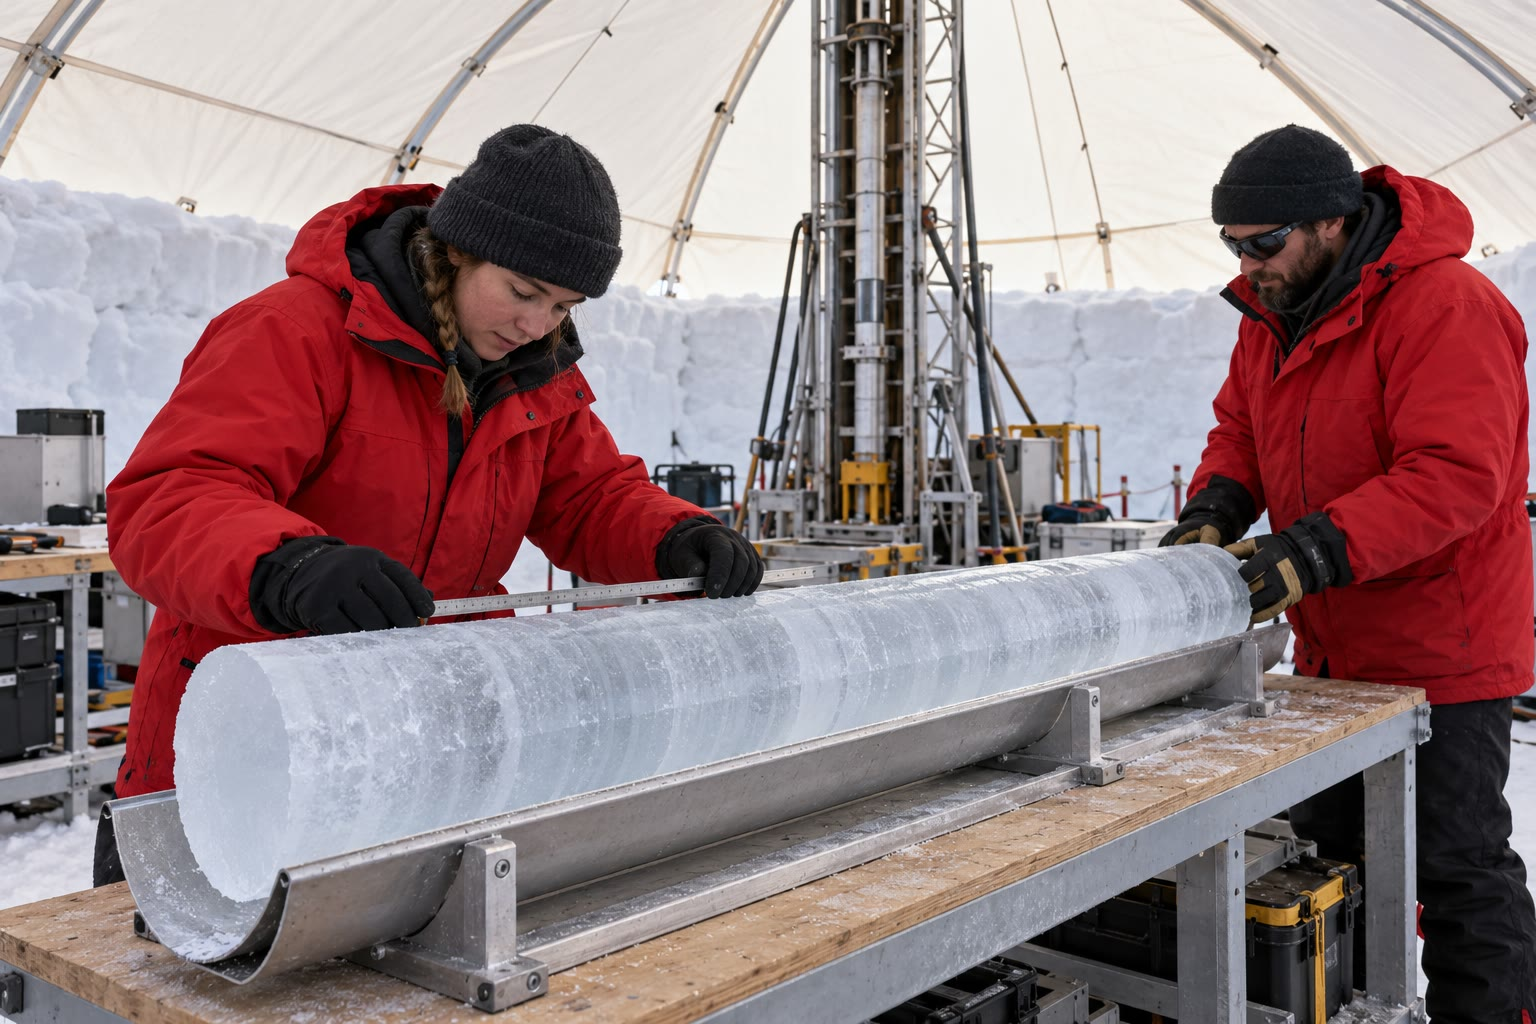
\includegraphics[width=\linewidth]{images/book5/ai/b3-ice-core-tent.jpg}

{\scriptsize Mengukur inti es dalam penyangga di dalam tenda pengeboran di atas
lembaran es, menara bor di belakang (ilustrasi buatan AI).}
\end{minipage}
\end{inthelab}

\section{Latihan}

\begin{exercise}[$\star$]\label{exo:b3:stable-isotopes:1}
Kalsit memiliki $\delta^{18}\mathrm O = \qty{30.5}{\permil}$ dan air tempat ia tumbuh
\qty{-2.1}{\permil}, keduanya terhadap VSMOW. Hitung $\alpha$, $1000\ln\alpha$ dan
$\Delta$. Seberapa besar selisih kedua nilai terakhir itu?
\end{exercise}

\begin{exercise}[$\star$]\label{exo:b3:stable-isotopes:2}
Sebuah stasiun pesisir lintang tinggi memiliki suhu tahunan rata-rata
\qty{-25}{\celsius}. Dengan hubungan dalam bab ini untuk stasiun seperti itu,
perkirakan $\delta^{18}\mathrm O$, $\delta\mathrm D$ dan \omterm{def:b3:stable-isotopes:d-excess}{kelebihan deuterium} dari
presipitasinya.
\end{exercise}
% ledger: dansgaard64:effects

\begin{exercise}[$\star$]\label{exo:b3:stable-isotopes:3}
Di sebuah cekungan, karbonat memiliki $\delta^{13}\mathrm C = \qty{+1.0}{\permil}$ dan materi organik
bernilai \qty{-26.0}{\permil}. Dengan masukan pada \qty{-5}{\permil}, hitung
$f_{\mathrm{org}}$.
\end{exercise}
% ledger: planavsky22:forg

\begin{exercise}[$\star$]\label{exo:b3:stable-isotopes:4}
Sebuah cangkang brakiopoda memiliki $\Delta_{47} = \qty{0.600}{\permil}$. Dengan kalibrasi
dalam bab ini, pada suhu berapa cangkang itu tumbuh?
\end{exercise}
% ledger: isogeochem:d47

\begin{exercise}[$\star\star$]\label{exo:b3:stable-isotopes:5}
Uap meninggalkan samudra pada $\delta^{18}\mathrm O = \qty{-13}{\permil}$ dan
mengendap sebagai hujan dengan $\alpha = 1.0100$ konstan. Berapa pecahan uap yang tersisa ketika
uap mencapai \qty{-33}{\permil}? Berapa $\delta^{18}\mathrm O$ hujan
saat itu?
\end{exercise}
% ledger: white13c9:rayleigh

\begin{exercise}[$\star\star$]\label{exo:b3:stable-isotopes:6}
Salju pada \qty{-40}{\permil} dibandingkan dengan air samudra pada 0. Hitung $\alpha$,
$1000\ln\alpha$, $1000(\alpha - 1)$ dan $\Delta$ di antara keduanya. Manakah dari
pendekatan proposisi yang gagal, dan dengan berapa besar?
\end{exercise}

\begin{exercise}[$\star\star$]\label{exo:b3:stable-isotopes:7}
Sebuah foraminifera memiliki $\delta^{18}\mathrm O = \qty{+1.50}{\permil}$ terhadap VPDB dan tumbuh di dalam
air pada \qty{0.00}{\permil} terhadap VSMOW. Hitung suhu tumbuhnya dengan
metode dalam bab ini, dan seberapa besar kesalahan \qty{0.1}{\permil} pada air
mengubahnya.
\end{exercise}
% ledger: isogeochem:ko97

\begin{exercise}[$\star\star$]\label{exo:b3:stable-isotopes:8}
Tumpukan bentik berubah sebesar \qty{1.77}{\permil} dari masa kini hingga
Maksimum Glasial Terakhir. Hapus bagian volume es yang dihitung dalam bab ini dan
ubah sisanya menjadi perubahan suhu air dalam, dengan menggunakan kemiringan
kalibrasi kalsit di sekitar \qty{2}{\celsius}.
\end{exercise}
% ledger: data:lr04, white13c9:ice-volume, isogeochem:ko97

\begin{exercise}[$\star\star$]\label{exo:b3:stable-isotopes:9}
Sebuah pirit memiliki $\delta^{34}\mathrm S = \qty{10.0}{\permil}$ dan $\delta^{33}\mathrm S =
\qty{8.2}{\permil}$. Hitung $\Delta^{33}\mathrm S$. Apa yang dikatakannya tentang
atmosfer saat pirit terbentuk?
\end{exercise}
% ledger: white13c9:s-mif

\begin{exercise}[$\star\star\star$]\label{exo:b3:stable-isotopes:10}
Dalam kondensasi sistem tertutup, uap dan seluruh kondensat yang terbentuk tetap
bersama dalam kesetimbangan. Tunjukkan bahwa uap kemudian memiliki $R_v/R_{v,0} = 1/[f +
\alpha(1 - f)]$, dan bandingkan dengan \omterm{prop:b3:stable-isotopes:rayleigh-distillation}{distilasi Rayleigh} untuk $f = 0.2$ dan
$\alpha = 1.01$.
\end{exercise}

\begin{exercise}[$\star\star\star$]\label{exo:b3:stable-isotopes:11}
Dari taksiran bahwa \qty{2000}{Gt} karbon metana pada
\qty{-60}{\permil} menggeser karbon yang dapat dipertukarkan sebesar \qty{-2.5}{\permil},
tentukan massa reservoir yang tersirat, dengan $\delta_0 = 0$. Dengan massa itu, berapa banyak
karbon organik pada \qty{-25}{\permil} menghasilkan pergeseran yang sama? Bandingkan dengan
rentang yang dipublikasikan.
\end{exercise}
% ledger: dickens11:petm

\begin{exercise}[$\star\star\star$]\label{exo:b3:stable-isotopes:12}
Tunjukkan bahwa, sepanjang lintasan pendinginan, $\mathrm d\delta_v/\mathrm dT = (\alpha - 1)(1000 +
\delta_v)\,\mathrm d\ln e_s/\mathrm dT$. Pada \qty{-20}{\celsius}, tempat
uap dari model dalam bab ini memiliki $\delta^{18}\mathrm O = \qty{-49.1}{\permil}$
dan kurva sublimasi memberikan $\mathrm d\ln e_s/\mathrm dT =
\qty{0.0960}{K^{-1}}$, hitung kemiringan ini.
\end{exercise}
% ledger: gkinis14:alpha-ice, iapws:melt-subl

\section{Soal: Perjalanan Setetes Hujan ke Dome Ilse}

\begin{problem}[{Soal akhir pekan --- isotop salju sepanjang sebuah
jalur buatan, paleosuhu dan ekskursi isotop karbon}]\label{pb:b3:stable-isotopes:1}
Massa udara meninggalkan tepi lembaran es rekaan pada \qty{0}{\celsius}
dengan uap bernilai $\delta^{18}\mathrm O = \qty{-20.0}{\permil}$ dan $\delta\mathrm D =
\qty{-150}{\permil}$, dan mendingin pada tekanan tetap saat bergerak ke pedalaman.
Salju terbentuk di stasiun Coast pada \qty{-10}{\celsius}, di Midway pada
\qty{-20}{\celsius} dan di Dome Ilse pada \qty{-30}{\celsius}, ketika pecahan
uap yang tersisa adalah $f = 0.425$, $0.169$ dan $0.0622$. Gunakan faktor fraksionasi es--uap
dalam bab ini, tetap sepanjang setiap ruas pada nilai
suhu pertengahannya.
% ledger: gkinis14:alpha-ice, iapws:melt-subl, dansgaard64:effects, isogeochem:ko97, isogeochem:d47, white13c9:ice-volume, data:lr04, planavsky22:forg, dickens11:petm

\medskip\noindent\textbf{Bagian I --- Distilasi.}
\begin{enumerate}
\item Hitung $\alpha^{18}$ dan $\alpha^{\mathrm D}$ pada $-5$, $-10$, $-15$, $-20$,
$-25$ dan \qty{-30}{\celsius} (lima angka penting untuk oksigen, empat untuk
deuterium).
\item Hitung $\delta^{18}\mathrm O$ uap saat tiba di Coast.
\item Hitung nilai untuk salju Coast.
\item Ulangi untuk Midway (rasio ruas $f$ adalah $0.169/0.425$).
\item Ulangi untuk Dome Ilse.
\item Berapa pecahan oksigen-18 asli dalam uap yang masih berada di udara
di Dome Ilse?
\end{enumerate}

\medskip\noindent\textbf{Bagian II --- Suhu dan deuterium.}
\begin{enumerate}[resume]
\item Hitung kemiringan $\delta^{18}\mathrm O$ salju terhadap
suhu kondensasi dari Coast ke Dome Ilse.
\item Berapa suhu permukaan tahunan rata-rata yang akan diberikan hubungan
stasiun Greenland kepada salju Dome Ilse? Mengapa itu bisa berbeda dari
\qty{-30}{\celsius}?
\item Hitung $\delta\mathrm D$ salju di ketiga stasiun dengan cara yang sama.
\item Hitung \omterm{def:b3:stable-isotopes:d-excess}{kelebihan deuteriumnya}. Bagaimana nilainya berubah ke arah pedalaman?
\item Apakah salju Dome Ilse berada pada garis air meteorik? Apa yang
tidak dimasukkan model tetapi ada dalam pembentukan salju sungguhan?
\end{enumerate}

\medskip\noindent\textbf{Bagian III --- Foraminifera di lepas pesisir.} Sebuah
inti sedimen di lepas pesisir memberikan foraminifera bentos dengan \qty{3.25}{\permil}
VPDB di bagian atas dan \qty{5.02}{\permil} pada Maksimum Glasial Terakhir; air dasar
\qty{0.00}{\permil} VSMOW saat ini.
\begin{enumerate}[resume]
\item Hitung suhu air dasar saat ini dengan
kalibrasi kalsit.
\item Hitung suhu glasial dengan asumsi air tidak berubah. Apakah
hasil itu mungkin?
\item Koreksi air glasial terhadap penurunan permukaan laut sebesar \qty{125}{m} dan
hitung ulang. Berapa pendinginan glasial air dasar?
\item Hitung $\Delta_{47}$ yang diharapkan pada kedua suhu itu dan
selisihnya.
\item Mengapa termometer \omterm{def:b3:stable-isotopes:clumped}{isotop menggumpal} tidak memerlukan komposisi
air?
\end{enumerate}

\medskip\noindent\textbf{Bagian IV --- Ekskursi isotop karbon.} Lebih dalam pada inti,
karbonat bernilai \qty{+0.5}{\permil} terputus oleh ekskursi singkat menuju
\qty{-3.0}{\permil}.
\begin{enumerate}[resume]
\item Sebelum ekskursi, dengan $\delta_{\mathrm{in}} = \qty{-5}{\permil}$ dan
$\Delta_B = \qty{-28}{\permil}$, hitung $f_{\mathrm{org}}$.
\item Ambil reservoir pada latihan~11, \qty{46000}{Gt} pada 0. Berapa banyak karbon
yang dibutuhkan ekskursi jika sumbernya metana pada \qty{-60}{\permil}?
\item Bagaimana jika sumbernya karbon organik pada \qty{-25}{\permil}?
\item Bagaimana jika sumbernya karbon mantel pada \qty{-5}{\permil}?
\item Observasi mana pada inti yang sama dapat membantu memilih di antara
sumber-sumber itu?
\item Nyatakan $\delta^{18}\mathrm O$ salju yang turun di Dome Ilse.
\end{enumerate}
\end{problem}
